\documentclass[]{article}
\usepackage{graphicx}
\usepackage{caption}
\usepackage{subcaption}
%opening
\title{ECE 657A Assignment \#2}
\author{Yuzhou Wang (20609396), Laura McCrackin (20262085), \newline and Huang Tianhui (20587328)       }


\begin{document}

\maketitle


%%\begin{figure}
%\includegraphics{../images/741741}
%%\end{figure}

\section{Parameter Selection and Classification}
Classify dataset D using five classifiers: k-NN, Support Vector Machine (with RBF kernel), Naïve Bayes Classifier, Decision Trees and Neural Networks. 
\subsection{Preprocessing}
%1)Preprocess the given data using the Z-score normalization, and split the data into two halves, the first half being the training set and the second half being the test set. (Normally you would do this randomly, but for this assignment a deterministic split will make the rest of the answers easier to grade).

For the original dataset D, we noticed that there are no missing values, and all the values are around the mean.  Therefore, we do not perform any outlier correction, and simply use Z-score normalization.  We used the first half of our data as training points, and the second half for testing.

%and use the function “zscore” in Matlab library directly.
%(Here later maybe I could add some comparation for different methods like after the normalization the graph is more in the center area)


\subsection{K-NN}
%2)For k-NN you need to evaluate the best value k to use. Using 5-fold cross validation (the crossvalind function can help) on the training set evaluate k-NN on the values k=[1, 3, 5, 7, ..., 31]. Plot a figure that shows the relationship between the accuracy and the parameter k. Report the best k in terms of classification accuracy.


Here we could see these two pictures for K-NN, and some different result could get. 
From the picture, we could see that the best k is 7 with around 73\% accuracy and sometimes k is 5 with nearly 72\% accuracy. After we run it for several times, we could the conclusion that the best k is between 5 and 12.
We could also see from the picture that at the very beginning, the accuracy increased and later after the best k, it decreased. I think maybe it is the reason that less than k points is to small to be a class, in other words, less points can not represent a class, but if K is too large, then it means that some other useless points maybe included which leads to a lower accuracy. Lastly, since we randomly choose the dataset and split them so that there could be some flexible results also.(seems not for we choose the beginning and later part)
And what is more, we should also notice about the accuracy about the dataset itself, maybe there are some outliers. And what is more, since it is DNA sequence, it means some cuts maybe represent nothing, but it still appears at the dataset with a label. Above all, the result we get is not the exactly right answer.


\begin{figure}[h]
\centering
  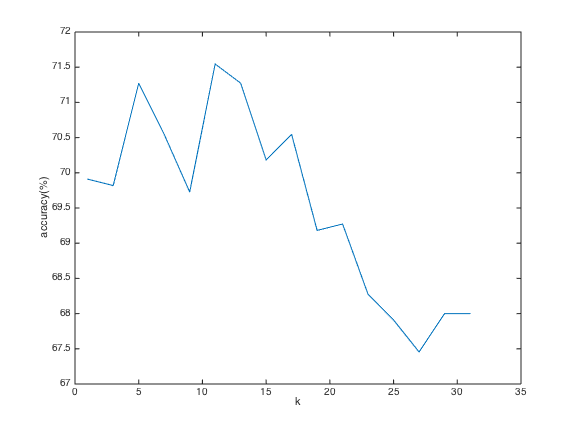
\includegraphics[width=1\linewidth]{../images/K-NN}
  \caption{The cross-validation accuracy using different values of k.}
  \label{fig:K-NN}

\end{figure}

\subsubsection{SVM Using RBF Kernel}
%3)For the RBF kernel SVM, there are two parameters to be decided: the soft margin penalty term "c" and the kernel width parameter “gamma”. Again use 5-fold cross validation on the training set to select the parameter "c" from the set [0.1, 0.5, 1, 2, 5, 10, 20, 50] and select the parameter “gamma” from the set [0.01, 0.05, 0.1, 0.5, 1, 2, 5, 10]. Report the best parameters in terms of classification accuracy including plotting the ROC curves.



Since the purpose of SVM is to produce a classifier that will work well on unseen examples (generalizes well), so it belongs to the decision (function) boundary approach 
(I am thinking it could be better if we plot a graph about the accuracy for different c and gamma and with the table result we could better demonstrate instead of only look at ROC graph) 
From the figure or table above, we could found that the highest accuracy appears for (which c and which gamma)
(Here should insert a picture of ROC)
as we could see from the ROC piture, we could see that both the trueth positive and false positive increase with (?), it means that(?)
What is more, theoretically with the increasing of gamma(kennel width), the accuracy decrease, because if the gamma is small enough(nearly 0), then it means that data point is not influenced or correlated with other data points. Small kernel width may cause over-fitting, and large one under-fitting. The so-called optimal kernel width is merely selected based on the tradeoff between under-fitting loss and over-fitting loss.

?I am not sure if we better to plot a gamma graph to demonstrate this point of view.?


\subsubsection{Comparing K-NN, SVM with an RBF kernel, Naive Bayes, Decision Trees, and Neural Networks }
%4)Using the chosen parameters from the above parameter selection process for k-NN and SVM, and the default setups for Naïve Bayes classifier, Decision Tree and Neural Network, classify the test set. Repeat each classification method 20 times by varying the split of training-test set (now select a random half of the data for training and the other half for test). Report the average and standard deviation of classification performance on the test set regarding: accuracy, precision, recall, and F- Measure. Also report the training time and classification time of the four methods.



From the accuracy table above, we could see that the best method is decision tree with the highest accuracy, precision,recall and F-measure but it is also the waste most of time to decide. The worst answer result is from K-NN method.


here should insert a table


\subsubsection{Strengths and Weaknesses of Each Method}
%5)Comment on the obtained results, what are the benefits and weaknesses of each method on this dataset. How could this analysis help to make the choice of the right method to use for a dataset of this type in the future?


K-NN: Training a k-NN classifier simply consists of determining k and preprocessing documents. In fact, if we preselect a value for k and do not preprocess, then kNN requires no training at all. It means that for K-NN, there is no training process and for the classification process, compare the test sample with all of the samples, the time measure has been divided by all of samples.
But the disadvantage of K-NN is that irrelevant dimensions could have bad influence a lot.

For SVM: For linear SVMs, at training time you must estimate the vector w and bias b by solving a quadratic problem, and at test time prediction is linear in the number of features and constant in the size of the training data. For kernel SVMs, at training time you must select the support vectors and at test time your complexity is linear on the number of the support vectors (which can be lower bounded by training set size * training set error rate) and linear on the number of features (since most kernels only compute a dos product; this will vary for graph kernels, string kernels, etc).

So from the above the SVM maybe the time consuming most.
Naïve Bayes Classifier: As we could conclude from the table that it is the most efficient method, linearly proportional to the time needed to just read in all the data.

Decision Trees: Decision trees are easy to use compared to other decision-making models, but preparing decision trees, especially large ones with many branches, are complex and time-consuming affairs.
Computing probabilities of different possible branches, determining the best split of each node, and selecting optimal combining weights to prune algorithms contained in the decision tree are complicated tasks that require much expertise and experience.
Decision trees moreover, examine only a single field at a time, leading to rectangular classification boxes. This may not correspond well with the actual distribution of records in the decision space.
In reality, the complexity in creating large decision trees mandates people involved in preparing decision trees having advanced knowledge in quantitative and statistical analysis. This raises the possibility of having to train people to complete a complex decision tree analysis. The costs involved in such training makes decision tree analysis an expensive option, and remains a major reason why many companies do not adopt this model despite its many advantages. But the advantage of this method is it provide easy way to view illustrations.


Neural Networks:  SVMs contain an underlying optimization step that is solved heuristically, so for any actual algorithm that purports to solve SVMs, the answer is undefined. A number like
O(n*n*n)is generally bandied around for implementations like libsvm, which means something like time/iteration * number of iterations (where numbr of  iterations is assumed to be constant)



\section{Clustering Analysis (for dataset F)}
The data has already been normalized into the range of [-1, 1], the sample labels are used for the purpose of performance evaluation.
Apply PCA to reduce the dimension to be 4, and then conduct the following clustering analysis.
\subsection{question 1}
1) Perform hierarchical clustering using agglomerative algorithms:
a) Stop when the number of clusters is 10 (the same as the number of given classes). Compare the linkage methods of “single”, “complete”, and “ward (minimum variance algorithm)”. Evaluate the clustering results in terms of Separation-Index, Rand-Index, and F-measure. Compare the three linkage types and comment.


For clustering data into 10 classes, we could use the matlab library function “clusterdata” and for three methods we could also add the keywords in the function:” linkage”, “complete”, “ward”
(here should add the result)
For calculating the rand-index, we are based on the function (a+b)/M
For separation-index calculation, we use the function:   
For F-measure function, we use the function F(i,j) = 2*precision(i,j)* recall(i,j)/(precision(i,j)+recall(i,j))


And according to the definition, we could get the conclusion that the result of separation-index is highly depending on the cluster result. Smaller separation-index means that every point in the cluster is close and as a result there could be more groups.
The result of rand-index and f-measure could have the similar trend for representing accuracy of the same cluster group, which is corresponding different with separation-index. It means that if there is a higher accuracy for cluster, the rand-index and f-measure could correspondingly higher, but it means larger size of cluster, as a result separation-index could be lower.



results are listed below:
For linkage method=single
Separation-Index=
Rand-Index=?
F-measure= ?
For linkage method=complete
Separation-Index=
Rand-Index=
F-measure=
For linkage method=ward
Separation-Index=
Rand-Index=
F-measure= 
above all of the result, we could get the conclusion that ???? method has the best perfomance. But we should not seperate to see the result, only depending on one method like only focus on rand-index or separation can not get the right results, combine together.
And from the table above we could get a conclusion that which method is good from which point of view.
Notice that the method we choose could influence the final result, maybe try for single and complex method both for calculate?
b) Fix the linkage type as “ward”, study the number of clusters from 2 to 15, increment by 1, what is the optimal number of clusters suggested by Separation- Index in this case?
Here from the figure below, we could get the conclusion that the best number of cluster is number.
For IS part, later added.
\subsection{question 2}
2) Cluster the data using k-means algorithm.
a) Run the algorithm for the number of clusters k from 2 to 15, increment by 1. Evaluate the clustering results in terms of Separation-Index, Rand-Index, and F-measure.


The algorithm of k-means could be run by the function “kmeans”, and we could see the picture for 2-2-(a). We could see that both rand-index increase a lot with the increasing number of cluster, and f-measure increase a lot at the beginning and later a little bit decrease.
And the reason why f-measure increase at the beginning is that, it is more close to the right cluster, and after the best cluster number, the false positive increase a lot, which makes it decrease later.

The reason why rand-index increase is because of the calculating function with the increasing number of cluster, it more close to the right cluster way, but for the value of M it did not change, so we could get the above result. (? not sure for this part analysis is right)

b) Plot these evaluation measures with respect to the number of clusters. What is the optimal number of clusters suggested by these indexes?

From the above pictures, the best cluster number is ??

\subsection{question 3}

3) Cluster the data using fuzzy c-means algorithm, with number of clusters as 10, and the fuzzy parameter (the exponent for partition matrix) m = 2.

a) Plot the average cluster membership values for the samples of the digit ‘1’ and ‘3’; explore their overlaps with other clusters.

For the picture 2-3-(a)-1 and 2-3-(a)-2 we could already plot the graph.
Here we could notice that there are more overlaps in cluster 3 but less in cluster 1.
Here just a little confused about why cluster 1 has less cluster. 
 
 
b) If we produce hard clustering by making the max membership value of a sample to be one and the rest of its membership values zero, evaluate the clustering results. Comment on the obtained results.

In hard clustering, data is divided into distinct clusters, where each data element belongs to exactly one cluster. In fuzzy clustering (also referred to as soft clustering), data elements can belong to more than one cluster, and associated with each element is a set of membership levels. 
For Fuzzy c-means
Separation-index=?
Rand-Index=?
F-measure=?
For k-means
Separation-index=?
Rand-Index=?
F-measure=?
For agglomerative algorithms
Separation-index=?
Rand-Index=?
F-measure=?
So from the above, we could get the conclution that, which method is the best, their advantages and disadvantages.

%\begin{figure}[p]
%\centering
%\begin{subfigure}{.5\textwidth}
%  \centering
%  \includegraphics[width=1\linewidth]{../images/hist9_before}
%  \caption{Feature 9}
%  \label{fig:sub1}
%\end{subfigure}%
%
%\begin{subfigure}{.5\textwidth}
%  \centering
%  \includegraphics[width=1\linewidth]{../images/hist24_before}
%  \caption{Feature 24}
%  \label{fig:sub2}
%\end{subfigure}
%\caption{Data histograms before normalization.}
%\label{fig:hist1}
%\end{figure}




































	

\begin{table}[h]
	\begin{center}
	 \caption{The accuracy and runtime for each feature selection method.}
	 \begin{tabular}{ | l | c | r  c  |}
	    \hline
	    Method & Average Accuracy (\%) & Runtime (s) &\\ 
	     &  & Feature Selection & Classification\\ 
	    \hline
	    
	    SFS Filter & 90.15 & 1.1696 & 0.0015 \\ 
	    SFS Wrapper & 91.82 & 0.2581 & 0.0014 \\
	    SBS Wrapper & 91.70 & 0.3587 & 0.0014\\
	    All 21 Features & 89.09 & -- & 0.0017\\
	    \hline    
	 \end{tabular}
	    \label{table:sfssbstable}
	\end{center}
\end{table}
\end{document}
